\documentclass[tikz,border=8pt]{standalone}
% Shared look for every TikZ diagram. Load with \input{../../tools/tikz-style.tex}
\usepackage[T1]{fontenc}
\usepackage{lmodern}
\renewcommand{\sfdefault}{lmr}  % diagrams use the same serif as the text
\usetikzlibrary{arrows.meta, positioning, shapes.geometric, calc, fit, backgrounds}
\definecolor{cblue}{HTML}{4C78A8}
\definecolor{corange}{HTML}{F58518}
\definecolor{cgreen}{HTML}{54A24B}
\definecolor{cred}{HTML}{E45756}
\definecolor{cpurple}{HTML}{B279A2}
\definecolor{cgrey}{HTML}{6B6B6B}
\tikzset{
  every picture/.style={font=\sffamily, line width=1.2pt},
  box/.style={draw=#1, fill=#1!12, rounded corners=4pt, align=center, inner sep=7pt, minimum height=1.1cm},
  box/.default=cgrey,
  arrow/.style={-{Stealth[length=3mm]}, draw=cgrey, line width=1.4pt},
  title/.style={font=\sffamily\bfseries\Large},
  note/.style={font=\sffamily\small, text=cgrey, align=center},
}
\AtBeginDocument{\hyphenpenalty=10000 \exhyphenpenalty=10000}

\begin{document}
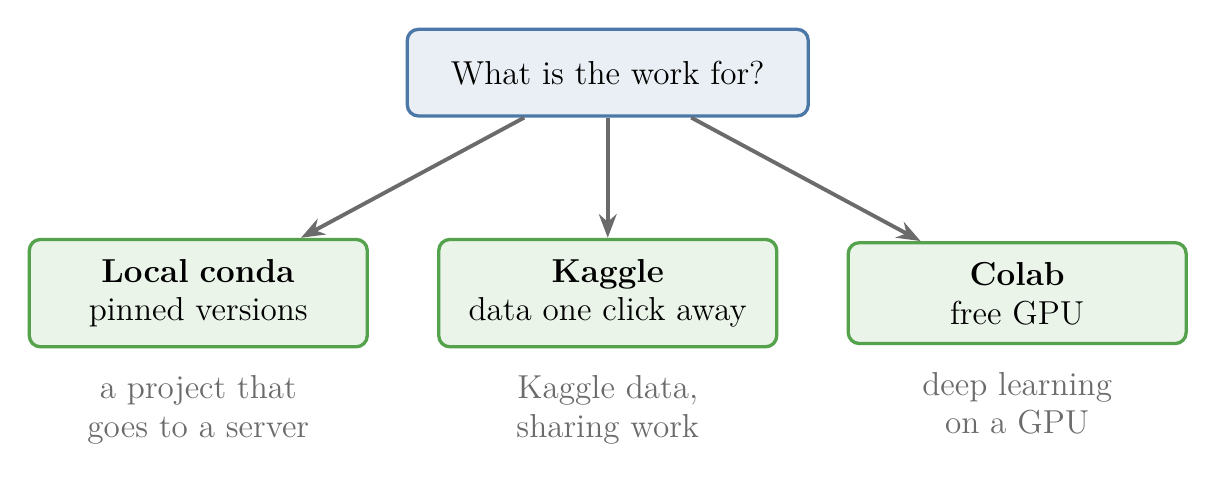
\begin{tikzpicture}[every node/.append style={font=\sffamily\large}]
\tikzset{note/.style={font=\sffamily\large, text=cgrey, align=center}}
  \node[box=cblue, text width=4.6cm] (q) at (0,0) {What is the work for?};
  \foreach \x/\n/\t/\w in {-5.2/l/{\textbf{Local conda}\\pinned versions}/{a project that\\goes to a server}, 0/k/{\textbf{Kaggle}\\data one click away}/{Kaggle data,\\sharing work}, 5.2/c/{\textbf{Colab}\\free GPU}/{deep learning\\on a GPU}} {
    \node[box=cgreen, text width=3.8cm] (\n) at (\x,-2.8) {\t};
    \draw[arrow] (q) -- (\n);
    \node[note, below=0.2cm of \n] {\w};
  }
\end{tikzpicture}
\end{document}
